\chapter{Resultados}
\label{c_resultados}

% Como crianças de 4 a 6 anos interagem com uma interface de programação focada em permitir visualizar os passos e a execução de um algoritmo? 
% Descrever como as crianças interagem com a interface de realidade aumentada

A análise vai ser apoiada pelo \autoref{quadro:equipes}. O \autoref{quadro:equipes} apresenta as equipes que participaram dos experimentos, com observações sobre características dos participantes. Estas observações foram elaboradas a partir da percepção do pesquisador e de falas das professoras. Além dessas características, o quadro demonstra o tempo de participação de cada equipe. O tempo de participação variou entre 13 e 35 minutos, devido a casos de não finalização da atividade. O tempo de 35 minutos, porém, foi suficiente para concluir todas as etapas, desde a ambientação os problemas de depuração. Outro fator de influência na duração da atividade foram troca de participantes, que entraram na brincadeira depois do início ou saíram antes do fim. Nesses casos, a equipe da criança é o grupo no qual ela permaneceu por mais tempo.

\begin{quadro}[!h]
    \caption{Equipes.}
    \label{quadro:equipes}
    \centering
    {
        \begin{footnotesize}
        {\renewcommand{\arraystretch}{1.2}
        \begin{tabular}{|l|l|l|p{11cm}|} 
            \hline
            \textbf{ Equipe/Tempo }                         & \textbf{Criança } & \textbf{Idade} & \textbf{Característica} \\ 
            \hline
            \multirow{2}{*}{Equipe 1. 35min}                & ID1               & 5:10                         & Menino curioso, comunicativo. Discordou de falas do pesquisador e dominou a brincadeira.                           \\ 
            \cline{2-4}
                                                            & ID2               & 5:7                          & Menino menos comunicativo que ID1, mas também falante. Preferiu não disputar o controle da brincadeira.            \\ 
            \hline
            \multirow{2}{*}{Equipe 2. 35min}                & ID3               & 5:10                         & Menina observadora. Preferiu não disputar o controle da brincadeira.                                               \\ 
            \cline{2-4}
            \multicolumn{1}{|c|}{}                          & ID4               & 5:11                         & Menina de personalidade forte. Procurou dominar o acesso ao brinquedo RoPE.                                        \\ 
            \cline{2-4}
            \multicolumn{1}{|c|}{}                          & ID5               & 6:0                          & A mais falante do grupo. Procurou disputar o controle do brinquedo.                                                \\ 
            \hline
            \multirow{2}{*}{Equipe 3. 24min}                & ID6               & 4:10                         & Considerado avançado para a idade. Compreendeu rápido o funcionamento da interface.                                \\ 
            \cline{2-4}
                                                            & ID7               & 3:11                         & Mais novo, ficou impressionado com o fato do brinquedo comer a maçã.                                               \\ 
            \hline
            Equipe 4. 13min                                 & ID8               & 4:3                          & Menino pouco comunicativo, distraído e carinhoso.                                                                  \\ 
            \hline
            \multirow{3}{*}{Equipe 5. 23min}                & ID9               & 4:7                          & Animado, comunicativo e observador.                                                                                \\ 
            \cline{2-4}
                                                            & ID10              & 4:8                          & Considerada de raciocínio rápido.                                                                                  \\ 
            \cline{2-4}
                                                            & ID11              & 4:8                          & Ansioso, animado e curioso. Entrou na metade da brincadeira.                                                       \\ 
            \hline
            \multirow{2}{*}{Equipe 6. 19min}                & ID12              & 4:2                          & Menina mais observadora que comunicativa. Esperava sua vez na brincadeira.                                         \\ 
            \cline{2-4}
                                                            & ID13              & 4:3                          & Menina recém iniciada no CDI. Ansiosa e comunicativa. Tentava pegar o brinquedo na mão.                            \\ 
            \hline
            \multirow{2}{*}{Equipe 7. 10min}                & ID14              & 4:10                         & Menina bastante comunicativa com as demais crianças.                                                               \\ 
            \cline{2-4}
                                                            & ID10              & 4:8                          & Da equipe 5. participou novamente aqui pois ID14 ficou sem dupla.                                                  \\ 
            \hline
            \multirow{2}{*}{Equipe 8. 30min}                & ID15              & 4:7                          & Menino pouco comunicativo, cuidadoso e observador. Precisou de auxílio da professora para entender a brincadeira.  \\ 
            \cline{2-4}
                                                            & ID16              & 4:5                          & Menina observadora. Não quis continuar na brincadeira até o final.                                                 \\ 
            \hline
            \multirow{2}{*}{Equipe 9. 20min}                & ID17              & -                            & Menina falante e brincalhona. Propôs novas trajetórias.                                                            \\ 
            \cline{2-4}
                                                            & ID18              & -                            & Menino agitado e ativo.                                                                                            \\ 
            \hline
            \multirow{2}{*}{Equipe 10. 22min}               & ID19              & -                            & Menino pouco comunicativo, observador. Concentrado nos botões.                                                     \\ 
            \cline{2-4}
                                                            & ID20              & -                            & Menino comunicativo e de respostas criativas.                                                                                    \\
            \hline
            \end{tabular}
        }
        \end{footnotesize}
    }
\end{quadro}

\section{Análise indutiva}

Esta seção a análise indutiva. 

\subsection{Interação com os blocos}

Após as etapas de seleção e ambientação, as crianças iniciaram o reconhecimento dos blocos. O pesquisador mostrou um bloco por vez, selecionado aleatoriamente, para as crianças dizerem seu significado. Essa etapa é importante pois a programação e a depuração dos algoritmos depende de compreender o significado dos blocos. 

De modo geral, as crianças entenderam as direções dos blocos, e demonstraram isso principalmente por meio de gestos com as mãos. O principal erro foi confundir as setas de “frente” e "trás" com “cima” e “baixo”. As respostas dadas com gestos indicaram mais erros de vocabulário do que de interpretação. Em 9 momentos as crianças usaram os termos “cima” ou “baixo” mas apontando para “frente” ou "trás", e apenas 1 criança realmente entendeu essas setas como sinais verticais. Para os blocos de “esquerda” e “direita”, as crianças usaram o termo “pro lado”, enquanto apontavam para a direção correta (\autoref{quadro:falas_simbolos}).

Além do reconhecimento dos símbolos dos blocos, duas falas evidenciam detalhes de design passíveis de melhoria. Na segunda fala do \autoref{quadro:falas_simbolos}, ID4 aponta o círculo da marca fiducial do bloco Frente e entende que o brinquedo está “rodando”. A criança respondeu certo logo em seguida, mas sua primeira percepção indica que a marca fiducial chamou sua atenção. Portanto o ideal seria eliminar a marca, pois ela não possui um significado útil para a criança. Em outro caso, a criança ID17 falou sobre o bloco Frente: \fala{Ele tá secando as mãos}. Uma possível origem desta resposta seria entender os quatro riscos desenhados no bloco Frente como símbolo de "vento". Essa criança compreendeu o significado correto posteriormente, mas sua fala indica que a imaginação fértil da criança, associada a pequenos detalhes de design, a fizeram obter uma conclusão inesperada.

\begin{quadro}[htbp]
    \captionquadro{Falas sobre os símbolos dos blocos.}
    \label{quadro:falas_simbolos}
    \begin{footnotesize}
    \begin{longtable}{ | m{.2\textwidth} | m{.7\textwidth} |}
        \hline
        \textbf{Bloco}  & \textbf{Falas e diálogos} \hline
        \endhead
        
        %%%%%%%%%%%%%%%%%%%
    
        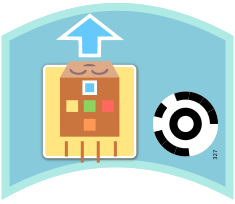
\includegraphics[width=.9\linewidth]{figs/blocks/frente.png} &
    
        \makecell{
            \falapessoa{ID2}{Ele tá botando... o sistema dele pra cima.} \\
            \falapessoa{ID1}{Ele tá olhando pra cima.} \\
            \\
            \falapessoa{ID4}{Rodando} \gesto{Aponta marca fiducial, que é redonda}\\
            \\
            \falapessoa{ID4 e ID5}{Pra aquele (lado)} \gesto{apontam para frente} \\
            \falapessoa{ID3}{Pra aquele} \gesto{aponta pra cima} \\
            \falapessoa{Pesquisador}{Pra cima?} \gesto{ID3 confirma com a cabeça} \\
            \\
            \falapessoa{ID10}{Uma flechinha} \\
            \falapessoa{Pesquisador}{Uma flechinha pra onde?} \\
            \falapessoa{ID10}{Pra cima} \gesto{aponta pra frente} \\
            \falapessoa{ID9}{Tipo daquelas ferramentas} \gesto{aponta brinquedos à frente} \\
            \\
            \falapessoa{Pesquisador}{O que ele tá fazendo aqui nesse desenho?} \\
            \falapessoa{ID13}{Dormindo!} \\
            \\
            \falapessoa{ID17}{Eu acho que ele tá secando as mãos... Eu acho que ele tá indo pra frente} \\
            \\
            \falapessoa{Pesquisador}{Esse bloquinho ele tá indo pra onde?} \\
            \falapessoa{ID15}{Pra pegar a maçã.}
        }

        \\ \hline

        %%%%%%%%%%%%%%%%%%%

        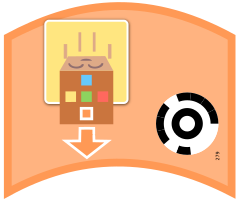
\includegraphics[width=.9\linewidth]{figs/blocks/tras.png} &

        \makecell{
            \falapessoa{ID1}{Esse aqui ele tá olhando pra baixo.} \\
            \\
            \falapessoa{ID10}{Pra baixo.}  \\
            \falapessoa{ID9}{Pra baixo!}  \\
            \falapessoa{Pesquisador}{E onde é pra baixo aqui no robô?} \\
            \falapessoa{ID10}{Grama} \gesto{Aponta para o chão}  \\
            \falapessoa{Pesquisador}{Qual é o botão que faz ele ir pra trás?} \\
            \falapessoa{ID9}{Aqui} \gesto{aponta botão trás} \\
            \\
            \falapessoa{ID17}{Ele tá indo pra trás} \\
            \falapessoa{ID5}{Pra baixo.} \\
            \falapessoa{ID4}{Esse aqui ele tá olhando pra baixo.} \\
        }

        \\ \hline

        %%%%%%%%%%%%%%%%%%%

        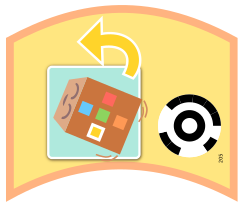
\includegraphics[width=.9\linewidth]{figs/blocks/esquerda.png} &

        \makecell{
            \falapessoa{ID2}{Ele tá olhando pra aquele lado.} \gesto{aponta para a esquerda} \\
            \falapessoa{ID5}{[tá rodando] pra aquele [lado].} \gesto{gira corpo para a esquerda} \\
            \falapessoa{ID10}{Esse aqui ó.} \gesto{aponta para a esquerda}
        }

        \\ \hline

        %%%%%%%%%%%%%%%%%%%

        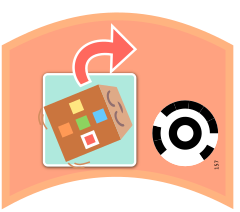
\includegraphics[width=.9\linewidth]{figs/blocks/direita.png} &

        \makecell
        {
            \falapessoa{ID2}{Esse aí ele tá olhando pro lado.} \gesto{aponta para a direita} \\
            \falapessoa{ID10}{Pro lado.} \gesto{aponta para botão do RoPE} \\
            \\
            \falapessoa{Pesquisador}{Ele tá fazendo alguma coisa?} \\
            \falapessoa{ID13}{Tá dormindo! Denovo.} \\
        }

        \\ \hline

        %%%%%%%%%%%%%%%%%%%

        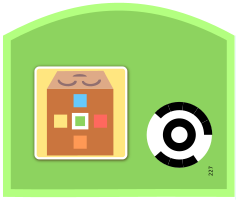
\includegraphics[width=.9\linewidth]{figs/blocks/inicio.png} &

        \makecell{
            \falapessoa{ID1}{Esse aqui também [está olhando pra cima].} \\
            \falapessoa{ID1}{Esse aqui é pra tirar vários.} \\
        }

        \\ \hline

        %%%%%%%%%%%%%%%%%%%

    \end{longtable}
    \end{footnotesize}
\end{quadro}

\begin{quadro}[!h]
   \begin{table_env}
   \caption{Reconhecimento dos blocos}
    \label{quadro:reconhecimentoblocos}
    \begin{tabular}{@{}l m{.6\textwidth} c@{}}
        \toprule
        Categoria                   & Descrição                                                                  & Frequência \\ \midrule
        "pro lado"                  & Aponta para a direção correta, mesmo não usando as palavras "direita"\ ou "esquerda"                                           & 5 \\
        "pra cima"                  & Fala ou aponta direção correta, mesmo falando outras palavras              & 4 \\
        Outros                      & Menciona algo não relacionado a movimento                                  & 3 \\
        "pra baixo"                 & Aponta ou fala a direção correta usando outras palavras                    & 2 \\
        Relaciona com o botão       & Aponta botão relacionado                                                   & 2 \\
        Menciona esquerda/direita   & Menciona palavras "esquerda" e "direita"\ durante reconhecimento dos blocos & 1 \\
        "pra trás"                  & Fala a palavra "trás"                                                      & 1 \\
        Rodando                     & Identifica botão frente ou trás como rodando                               & 1 \\
        Aponta pra cima             & Confunde frente com cima, apontando pra cima                               & 1 \\
        Pro chão                    & Diz que o brinquedo está indo pro chão, sem indicar a direção "trás"       & 1 \\ \nidrule
        Indo pegar a maçã           & Diz que o brinquedo está "Indo pegar a maçã"                               & 1 \\ \bottomrule
        \end{tabular}
   \end{table_env}
   \sourceauthor
\end{quadro}

O \autoref{quadro:reconhecimentoblocos} apresenta exemplos das respostas obtidas. Destaca-se a primeira fala, de ID2, que ao analisar o bloco Frente diz: \fala{ele está botando... o sistema dele pra cima}. Provavelmente a criança não sabe o que é um sistema, mas sabe que é algo associado a um robô. A dinâmica da atividade não permitiu investigar, naquele instante, qual o entendimento da criança sobre o tema, mas temas relacionados à computação apareceram posteriormente:

\begin{dialogo}
    \gesto{ID2 Clica diversas vezes em todos os botões} \\
    \falapessoa{ID1}{Para, senão ele vai \textbf{bugar}!} \\
    \falapessoa{Pesquisador}{Bugar? o que é bugar?} \\
    \falapessoa{ID1}{É quando ele faz assim ó} \gesto{ID1 e ID2 fazem posição de “estátua”.}
\end{dialogo}

Esta criança, portanto, entende que \destaque{bugar} é algo relacionado a travamentos e deve ser evitado. Outras crianças apresentaram outras justificativas quando o robô não se moveu: ID14 disse: \fala{Não anda esse robô. Tava dormindo, coitadinho}. O vocabulário "avançado"\ da Equipe 1 não apareceu nas outras equipes.

A Equipe 1, além de compreender o significado dos blocos, iniciou a exploração dos mesmos, relacionando-os uns com os outros. As crianças começaram a encaixar os blocos iguais entre si, formando 4 grupos de blocos (4 Frente, 2 Esquerda, 2 Direita, 2 Trás) (\autoref{fig:relacao_blocos}). O pesquisador questionou o motivo de tal agrupamento, conforme o diálogo a seguir:

\begin{dialogo}
    \gesto{Crianças encaixam os blocos} \\
    \falapessoa{Pesq}{Dá pra montar né? Dá pra encaixar}{01.59} \\
    \gesto{ID2 tenta encaixar peças de cores diferentes} \\
    \falapessoa{ID1}{Não, esse aqui não pode. Esse aqui não é desse.}{02.06} \\
    \falapessoa{ID2}{É um jogo…}{02.08} \\
    \falapessoa{ID1}{Esse aqui tá olhando pra baixo.}{02.11} \gesto{segura bloco Trás} \\
    \falapessoa{ID1}{Esse aqui vou conectar com esse, e esse conecta com esse}{02.20} \gesto{unindo peças de mesma cor} \\
    \falapessoa{Pesq}{Porque esses assim?}{02.30} \\
    \falapessoa{ID1}{Porque tão olhando pro mesmo lado né!}{02.32} \\
    \falapessoa{Pesq}{Ah... e pela cor né}{02.36} \\
    \falapessoa{ID1}{Não, porque tão olhando pro mesmo lado!}{02.40} \\
    \falapessoa{Pesq}{Ah... entendi...}{02.40}
\end{dialogo}

A justificativa para tal associação, portanto, foi a posição do brinquedo desenhado, e não cor do bloco. Percebendo a similaridade entre pares de blocos, ID1 sugeriu que poderia ser jogado o "Jogo da Memória". O pesquisador e os dois meninos então viraram os blocos com a face para baixo (\autoref{fig:jogo_memoria}), e, cada um a sua vez, virou duas peças.

\begin{figure}[!htbp]
    \begin{center}
    \begin{subfigure}{.5\textwidth}
        \centering
        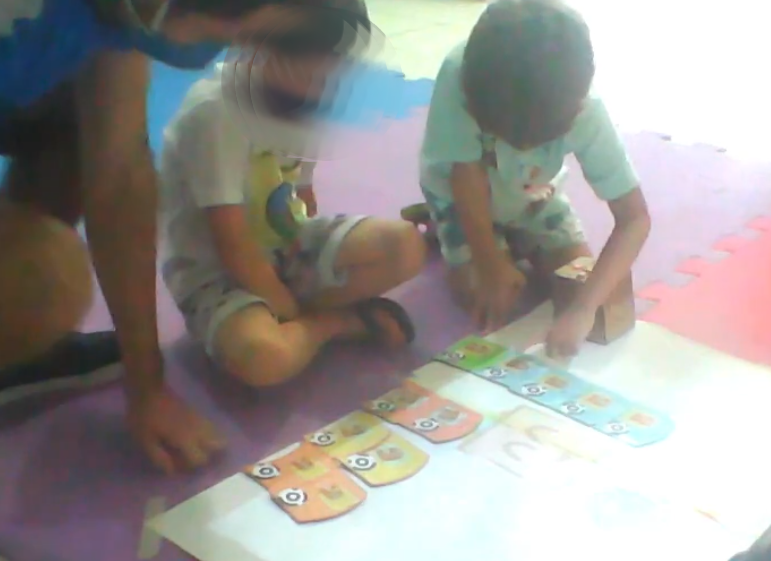
\includegraphics[width=.9\linewidth,fbox]{figs/relacao_blocos.png}
        \caption{Relacionamento entre blocos}
        \label{fig:relacao_blocos}
    \end{subfigure}%
    \begin{subfigure}{.4\textwidth}
        \centering
        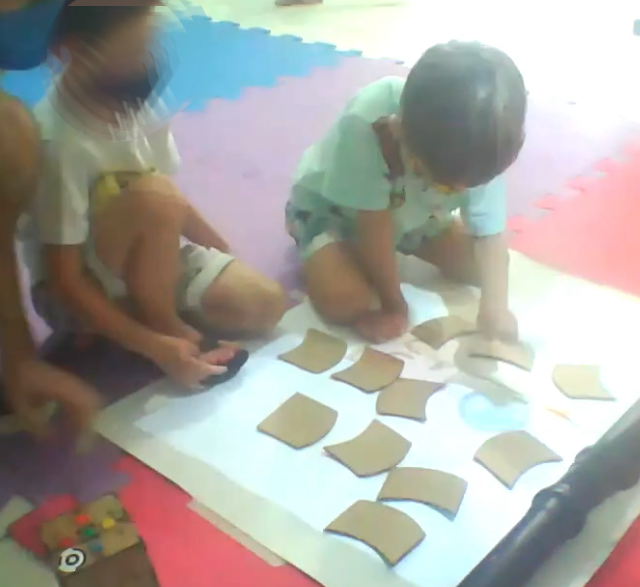
\includegraphics[width=.9\linewidth,fbox]{figs/jogo_memoria.png}
        \caption{Jogo da memória, proposto pela dupla}
        \label{fig:jogo_memoria}
    \end{subfigure}
    \end{center}
    \sourceauthor
    \label{fig:equipe1}
\end{figure}

Outro aspecto de design a ser melhorado apareceu durante o jogo: os blocos Direita e Trás tem cores muito parecidas (tons de vermelho e laranja). Ao procurar blocos iguais, ID2 virou um bloco Trás e um bloco Direita e considerou um ponto ganho. ID1 alertou o colega ao perceber o engano, e ID2 devolveu os blocos. O diálogo revela a interação entre as crianças durante o jogo:

\begin{dialogo}
    \falapessoa{ID2}{Agora é minha vez.}\gesto{vira peças vermelha e laranja, e pensa que acertou}{11.57} \\
    \falapessoa{ID1}{Errou, é diferente.}{12.00} \\ 
    \falapessoa{Pesq}{É diferente né. Mas é parecido, é parecido.}{12.05}
\end{dialogo}

A mesma situação ocorreu com ID8, que selecionou o bloco Trás ao tentar fazer o brinquedo girar à Direita. A Prof\_6 então atuou direcionando a atenção da criança para ela perceber o engano:

\begin{dialogo}
    \falapessoa{Pesq}{Viu que ele foi pra trás? Porque aqui tá o bloquinho laranja. O que ele tem que fazer?} \\
    \falapessoa{ID8}{Vermelho!} \\
    \falapessoa{Pesq}{E qual é o bloquinho vermelho?} \\
    \falapessoa{ID8}{Esse aqui ó} \gesto{pega o laranja} \\
    \falapessoa{Prof\_6}{Esse é vermelho, tem certeza? Olha bem...} \\
    \falapessoa{Pesq}{Qual é mais vermelho. Esse ou esse?} \gesto{coloca blocos esquerda e trás lado a lado} \\
    \falapessoa{Prof\_6}{Olha a flechinha se é igual.} \\
    \falapessoa{ID8}{Vermelho é esse.} \gesto{aponta bloco Direita} \\
\end{dialogo}

Esses dois diálogos demonstram que a interação com os objetos físicos viabilizou conversas de criança para criança e de professor para criança. Nos dois casos uma criança foi alertada por colega ou professor sobre um erro, e pode então desfazê-lo manipulando os blocos de papelão. No primeiro caso a correção do erro consistiu em virar a face dos blocos para baixo pois não formavam um par do jogo da memória. No segundo caso, a correção consistiu em encaixar outro bloco na sequência de blocos. Isso demonstra que ações similares surgiram tanto na brincadeira sugerida pelas crianças quanto na construção de um algoritmo. São ações naturais, presentes nas brincadeiras, mas que viabilizam o contato com conceitos de computação e \ac{PC}.

% \subsubsection{Associação dos blocos com os botões}


\subsection{Percepções de realidade aumentada}

O diferencial da RoPE AR para outros tipos de interface de programação é a união entre realidade aumentada e blocos tangíveis. Neste sentido, a questão é: como as crianças perceberam e interagiram com a RA?

Para respondê-la, a análise dos vídeos apontou alguns tipos de eventos em que as crianças perceberam os elementos projetados e os relacionaram com objetos reais. Para contar esses eventos, foram considerados gestos, falas e reações de animação ou estranhamento das crianças (\autoref{quadro:percepcao_ra}).

\begin{quadro}[!h]
    \begin{table_env}
    \caption{Eventos de percepção de realidade aumentada}
     \label{quadro:percepcao_ra}
     \begin{tabular}{@{}l m{.5\textwidth} c@{}}
        \toprule
        Categoria                                      & Descrição                                                                             & Frequência \\ \midrule
        Aponta para figura projetada                   & Criança aponta para uma figura projetada                                              & 32 \\
        Percebe que brinquedo "comeu"\ a maçã           & Criança fala ou gesticula indicando que o brinquedo "comeu"\ a maçã                   & 20 \\
        Levanta brinquedo, procurando maçã             & Criança levanta o brinquedo procurando a maçã que desapareceu                         & 13 \\
        Percebe que maçã apareceu                      & Criança aponta para a maçã que acabou de parecer                                      & 10 \\
        Estranha que não comeu maçã                    & Criança estranha quando o brinquedo não come a maçã ao chegar no quadrado dela        & 5 \\
        Percebe destaque do bloco                      & Criança aponta o bloco destacado pelo projetor                                        & 3 \\
        Tenta tocar no objeto virtual                  & Criança coloca a mão sobre a imagem de alguma figura projetada                        & 3 \\
        Coloca bloco sobre a maçã                      & Criança percebe a localização da figura projetada e coloca um objeto físico sobre ela & 2 \\
        Percebe um detalhe de uma figura projetada     & Menciona algum detalhe, como a folha da maçã                                          & 1 \\ \bottomrule
        \end{tabular}
    \end{table_env}
    \sourceauthor
 \end{quadro}

O evento mais frequente (32) foi as crianças apontarem para um objeto projetado, na maior parte dos casos a maçã. Ela era a figura principal do mapa projetado, a ser capturada pelo RoPE. Portanto, o fato de as crianças apontarem para ela apenas indica que ela estava suficientemente visível.
 
O evento a ser destacado, porém, foi as crianças levantarem o brinquedo RoPE e o virarem de “cabeça para baixo” após ele “comer a maçã”. Esse evento ocorreu por 13 vezes, em 5 equipes. Ele indica que as crianças tentaram entender se o destino da “maçã” foi a “barriga” do robô. Uma das crianças também olhou ao redor do mapa e procurou a maçã embaixo dos blocos de papelão. Esses eventos evidenciam que as crianças não conseguiram distinguir claramente os objetos reais e virtuais. 

\begin{figure}[!htbp]
    \centering
    \begin{subfigure}{.5\textwidth}
        \centering
        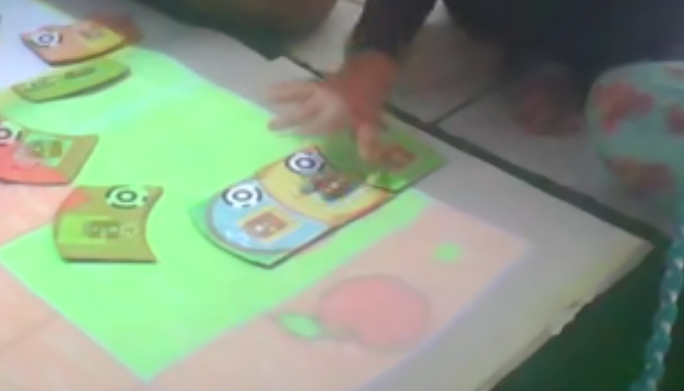
\includegraphics[width=.9\linewidth,fbox]{figs/percepcao_ra/mao_sobre_blocos.png}
        \caption{ID11 coloca a mão sobre os blocos}
        \label{fig:mao_sobre_blocos}
    \end{subfigure}%
    \begin{subfigure}{.5\textwidth}
        \centering
        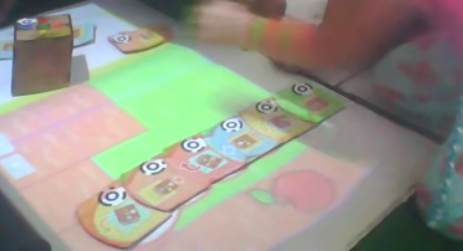
\includegraphics[width=.9\linewidth,fbox]{figs/percepcao_ra/sequencia_blocos.png}
        \caption{ID10 encaixa blocos para ver a iluminação}
        \label{fig:sequencia_blocos}
    \end{subfigure}
    \caption{Exploração dos blocos}
    \label{fig:percepcoes_ra}
\end{figure}

Outros exemplos de interação com a RA foram tentativas de segurar a maçã ou encostar nos círculos de destaque dos blocos. A Equipe 5, por exemplo, percebeu o destaque dos blocos que aparece quando um algoritmo válido é criado. No primeiro momento em que a equipe, de modo exploratório, criou um algoritmo e a RoPE AR o destacou, ID11 percebeu o destaque e aproximou a mão dos blocos (\autoref{fig:mao_sobre_blocos}). Em seguida, a colega ID10 entendeu que o encaixe dos blocos provocou sua iluminação. Como consequência, ID10 criou uma longa sequência de blocos para ver o efeito da iluminação sobre os mesmos  (\autoref{fig:sequencia_blocos}).

Essa ações indicam que a associação de elementos virtuais aos reais foi compreendida. Entretanto, essas ações ocorreram esporadicamente e as crianças rapidamente perderam o interesse ao perceber que esses objetos não eram manipuláveis. As crianças também não demonstraram interesse pelo destaque dos blocos durante a execução. Em apenas três momentos houve apontamentos para os blocos destacados e nenhuma fala sobre eles. Esse recurso serviu como um auxílio para o pesquisador explicar a sequência de execução dos blocos, mas não eliminou a necessidade de apontar os blocos com a mão.

Por fim, as crianças apresentaram interesse pela figura da maçã, que é uma entidade conhecida\footnote{Maçã é uma fruta presente nas refeições das crianças no CDI.}. Havia forte desejo de fazer o robô capturá-la. Para isso, as principais estratégias foram apertar os botões, mesmo que desativados, testar a combinação de diferentes blocos, e também empurrar o brinquedo com as mãos. O alcance do objetivo provocou reações de espanto e animação. Neste sentido, apesar de a tarefa ser repetitiva (sempre capturar a maçã), não se percebeu perda de engajamento. Pelo contrário, as crianças quiseram continuar a brincadeira mesmo após o término.

\section{Interação com os botões}

\section{Análise dedutiva}

%\section{}
% quanto tempo em cada fase?

% quanto tempo em cada estado?


%\section{Comparação com os trabalhos relacionados}
%\label{sec:comparacao}

% não tem limitação no número de blocos
% o formato dos blocos pode variar

%\section{Considerações}
%\label{sec:}

%Este capítulo pode ter uma última seção como esta denominada ``Considerações'' ou ``Discussão'' consolidando a análise dos resultados.
\section{Entrevistas}
















































































\begin{comment}

    %A força motriz do design iterativo são as metas do usuário, que são ações que o usuário deseja poder fazer \cite{rogers_design_2013}. Neste trabalho, o alcance das metas de usabilidade se dá quando a criança:
    
    \begin{itemize}
        \item posiciona o brinquedo na posição inicial;
        \item percebe que os blocos representam ações do robô;
        \item sequencia blocos formando um algoritmo;
        \item inicia execução do algoritmo;
        \item altera sequência de blocos; e
        \item percebe blocos destacados durante execução.
    \end{itemize}
    
    Para direcionar a observação, as categorias de análise serão 
    (i) para quais elementos da interface as crianças olham;
    (ii) se e como as crianças manipulam os blocos; 
    (iii) perguntas realizadas; 
    (iv) se e como as crianças comparam os blocos com os símbolos do robô; 
    (v) como ocorre o início da execução; 
    (vi) em que local e direção posicionam o robô; e 
    (vii) se e como os elementos virtuais são percebidos pelas crianças.
    
    %A colaboração será observada quando duas ou mais crianças brincarem em conjunto com os blocos. Esse tipo de evento já foi observado em estudos anteriores \cite{sapounidis_tangible_2019, raabe_estudo_2019}, mas precisa ser confirmado neste estudo para afirmar que a interface apresentada tem os benefícios das interfaces tangíveis. 
    
    % \cite{bardin_alise_1979}.
    \end{comment}